\section{Tests Environment and Results}

The previous section described how the system was implemented and how each
component interacts within the complete flow, from a user that uploads a file to
the leader performing the Corruption Check phase (showed in Section
\ref{sec:check-corruption}).

This section presents the testing environment, the scenarios used during evaluation, and the obtained results. The tests were executed on a cluster of nine machines running Ubuntu 24.04.1 LTS (GNU/Linux 6.8.0-51-generic x86\_64). The specifications of the virtual machines are summarized in Table \ref{tab:vms-specs}. The nodes were geographically distributed across the European continent.

\begin{table}[h!]
    \centering
    \begin{tabular}{|l|c|c|c|c|}
    \hline
       \textbf{Node ID} & \textbf{IPv4} & \textbf{CPU(s)} & \textbf{RAM} & \textbf{Disk} \\
       \hline
        GW & 51.15.221.121 & 8 & 32 GB & 45 GB \\
        Agent 1 & 212.47.241.22 & 4 & 16 GB & 45 GB \\
        Agent 2 & 51.15.138.169 & 4 & 16 GB & 45 GB \\
        Agent 3 & 51.159.178.75 & 4 & 8 GB & 45 GB \\
        Agent 4 & 51.158.75.32 & 4 & 8 GB & 45 GB \\
        Agent 5 & 51.158.233.202 & 4 & 8 GB & 45 GB \\
        Agent 6 & 51.15.108.2 & 4 & 8 GB & 45 GB \\
        Agent 7 & 151.115.42.176 & 4 & 8 GB & 45 GB \\
        Agent 8 & 151.115.104.48 & 4 & 8 GB & 45 GB \\
        \hline
    \end{tabular}
    \caption{Specifications of the machines used in the testing environment.}
    \label{tab:vms-specs}
\end{table}

Each test scenario considered four parameters:
\begin{itemize}
    \item \textbf{Number of agents}: total number of agents participating in the Reed-Solomon configuration of $n + k$ nodes.
    \item \textbf{Number of offline agents}: number of agents intentionally
        disconnected during the corruption check.
    \item \textbf{Number of files}: number of files included in the test.
    \item \textbf{File size}: size of each uploaded file. Since each file is divided into $n + k$ shards, the size of a single shard equals $\frac{\text{file size}}{\text{number of agents}}$ bytes.
\end{itemize}

After each upload, the environment was tested through the corruption check, measuring the total elapsed time in seconds from the initial check request to its completion. Each plot reports the average total elapsed time over three independent runs.

\paragraph{Test 1: Large files, all Agents online}

In the first scenario, 100 files of 100 MB each were uploaded, yielding a total
dataset of 10 GB. Each file was divided into $n+k$ shards and distributed across
the Agents in the cluster. All Agents remained online during the corruption
check. Figure \ref{fig:test-1} (top-left) shows the elapsed time for the corruption check as the number of Agents increases from 3 to 8. As expected, elapsed time grows with the number of Agents due to the increasing number of shard verifications. The elapsed time ranges from 1.373 seconds with 3 Agents to 23.892 seconds with 8 Agents. These results establish a baseline for moderate-size files, indicating that the system efficiently handles shard verification with minimal computational overhead.

\begin{figure}[!ht]
\centering
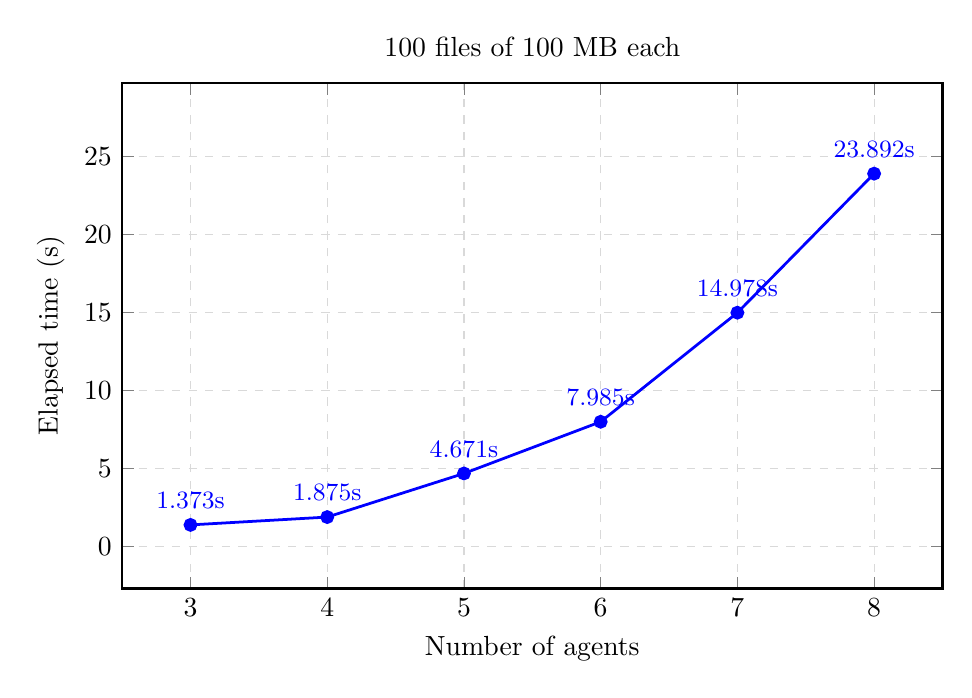
\begin{tikzpicture}
\begin{axis}[
    width=12cm, height=8cm,
    xlabel={Number of agents},
    ylabel={Elapsed time (s)},
    xmin=3, xmax=8,
    ymin=0, ymax=27,
    xtick={3,4,5,6,7,8},
    ytick={0,5,10,15,20,25},
    grid=major,
    grid style={dashed,gray!30},
    thick,
    title={100 files of 100 MB each},
    enlargelimits=0.1,
    clip=false,
    nodes near coords,
    every node near coord/.append style={font=\small, anchor=south, yshift=2pt},
    point meta=explicit symbolic
]

\addplot[color=blue, mark=*, line width=1pt] coordinates {
    (3,1.373) [1.373s]
    (4,1.875) [1.875s]
    (5,4.671) [4.671s]
    (6,7.985) [7.985s]
    (7,14.978) [14.978s]
    (8,23.892) [23.892s]
};
\end{axis}
\end{tikzpicture}
\caption{Elapsed time of the corruption check with 100 files, each 100 MB in size, 0 offline agents.}
\label{fig:test-1}
\end{figure}


\newpage
\paragraph{Test 2: Many small files, all Agents online}

The second test involved 10,000 files of 1 MB each, maintaining the same total
dataset size of 10 GB. This scenario highlights the impact of a high file count
relative to file size. As shown in Figure \ref{fig:test-2} (top-right), elapsed time increases substantially with the number of Agents, from 0.469 seconds with 3 Agents to 81.032 seconds with 8 Agents. The steep growth compared to Test 1 indicates that the number of files significantly influences corruption check performance, primarily due to the overhead of metadata operations and managing numerous small shards. The results suggest that for datasets with many small files, increasing the cluster size may yield diminishing returns, as coordination costs become more significant.

\begin{figure}[!ht]
\centering
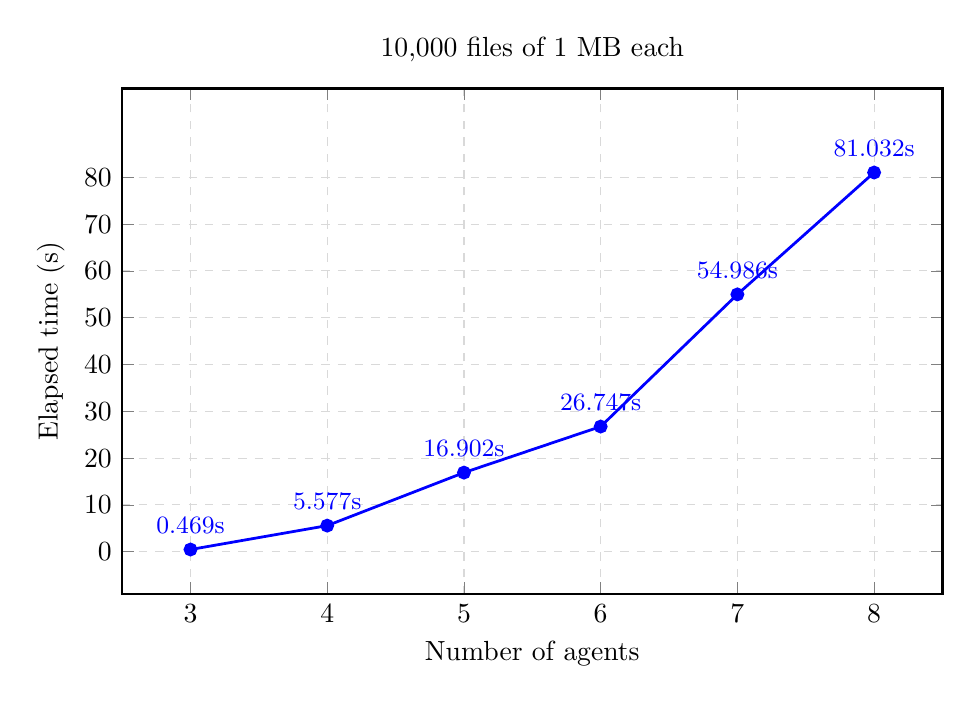
\begin{tikzpicture}
\begin{axis}[
    width=12cm, height=8cm,
    xlabel={Number of agents},
    ylabel={Elapsed time (s)},
    xmin=3, xmax=8,
    ymin=0, ymax=90,
    xtick={3,4,5,6,7,8},
    ytick={0,10,20,30,40,50,60,70,80},
    grid=major,
    grid style={dashed,gray!30},
    thick,
    title={10,000 files of 1 MB each},
    enlargelimits=0.1,
    clip=false,
    nodes near coords,
    every node near coord/.append style={font=\small, anchor=south, yshift=2pt},
    point meta=explicit symbolic
]

\addplot[color=blue, mark=*, line width=1pt] coordinates {
    (3,0.4685) [0.469s]
    (4,5.577) [5.577s]
    (5,16.902) [16.902s]
    (6,26.747) [26.747s]
    (7,54.986) [54.986s]
    (8,81.032) [81.032s]
};
\end{axis}
\end{tikzpicture}
\caption{Elapsed time of the corruption check with 10000 files, each 1 MB in size, 0 offline agents.}
\label{fig:test-2}
\end{figure}

\newpage
\paragraph{Test 3: Small files, partially offline Agents}

The third scenario evaluates the effect of offline Agents. 1,000 files of 150 KB
each were uploaded, and elapsed time was measured both with all Agents online
and with a subset of Agents offline during the corruption check.
Figure \ref{fig:test-3} (bottom-left) compares the two configurations. Offline Agents introduce additional latency due to shard reconstruction, with elapsed times ranging from 28.2 to 91.338 seconds, compared to 3.1 to 69.221 seconds when all Agents are online. The overhead is particularly pronounced at smaller cluster sizes, highlighting the computational cost associated with reconstructing missing shards. These results confirm that erasure coding ensures data availability despite node failures, albeit at a measurable performance cost.

\begin{figure}[!ht]
\centering
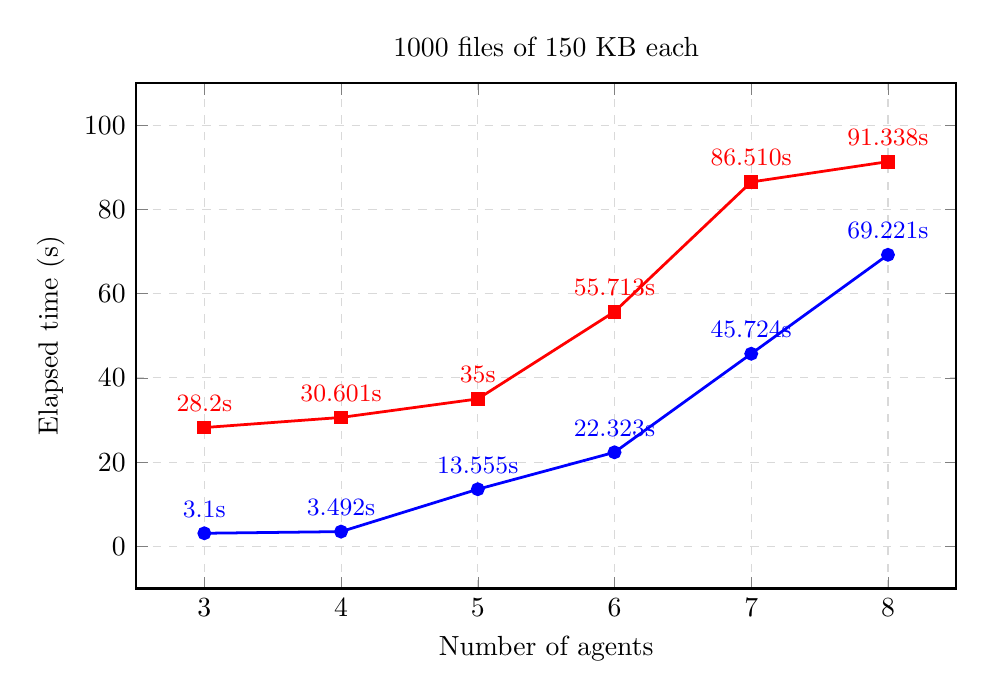
\begin{tikzpicture}
\begin{axis}[
    width=12cm, height=8cm,
    xlabel={Number of agents},
    ylabel={Elapsed time (s)},
    xmin=3, xmax=8,
    ymin=0, ymax=100,
    xtick={3,4,5,6,7,8},
    ytick={0,20,40,60,80,100},
    grid=major,
    grid style={dashed,gray!30},
    thick,
    title={1000 files of 150 KB each},
    enlargelimits=0.1,
    clip=false,
    nodes near coords,
    every node near coord/.append style={font=\small, anchor=south, yshift=2pt},
    point meta=explicit symbolic
]

% Online agents
\addplot[color=blue, mark=*, line width=1pt] coordinates {
    (3,3.1) [3.1s]
    (4,3.492) [3.492s]
    (5,13.555) [13.555s]
    (6,22.323) [22.323s]
    (7,45.724) [45.724s]
    (8,69.221) [69.221s]
};

% Offline agents
\addplot[color=red, mark=square*, line width=1pt] coordinates {
    (3,28.2) [28.2s]
    (4,30.601) [30.601s]
    (5,35) [35s]
    (6,55.713) [55.713s]
    (7,86.510) [86.510s]
    (8,91.338) [91.338s]
};

\end{axis}
\end{tikzpicture}
\caption{Elapsed time of the corruption check with 1000 files, each 150 KB in
    size. In blue 0 offline agents; in red with offline
    agents.}
\label{fig:test-3}
\end{figure}

\newpage
\paragraph{Test 4: Very large number of tiny files}

The fourth test examines system behavior with an extremely large number of very
small files. The dataset consisted of 1,000,000 files, distributed in two
configurations: 3-byte files across 3 Agents and 4-byte files across 4 Agents.
Figure \ref{fig:test-4} (bottom-right) shows that the corruption check completes in under 5 minutes for both configurations, demonstrating scalability for large file counts. Interestingly, adding an additional Agent increases elapsed time by approximately 14\%, suggesting that the coordination overhead of an extra node outweighs marginal benefits for extremely small files. While the total data volume is minimal (3-4 MB), elapsed times are substantial, confirming that metadata operations and shard tracking dominate the performance cost in this scenario. These results indicate that the system can efficiently handle real-world workloads involving millions of small objects, such as IoT sensor data or fragmented logs, though careful consideration of cluster size is necessary for optimal performance.

\begin{figure}[!ht]
\centering
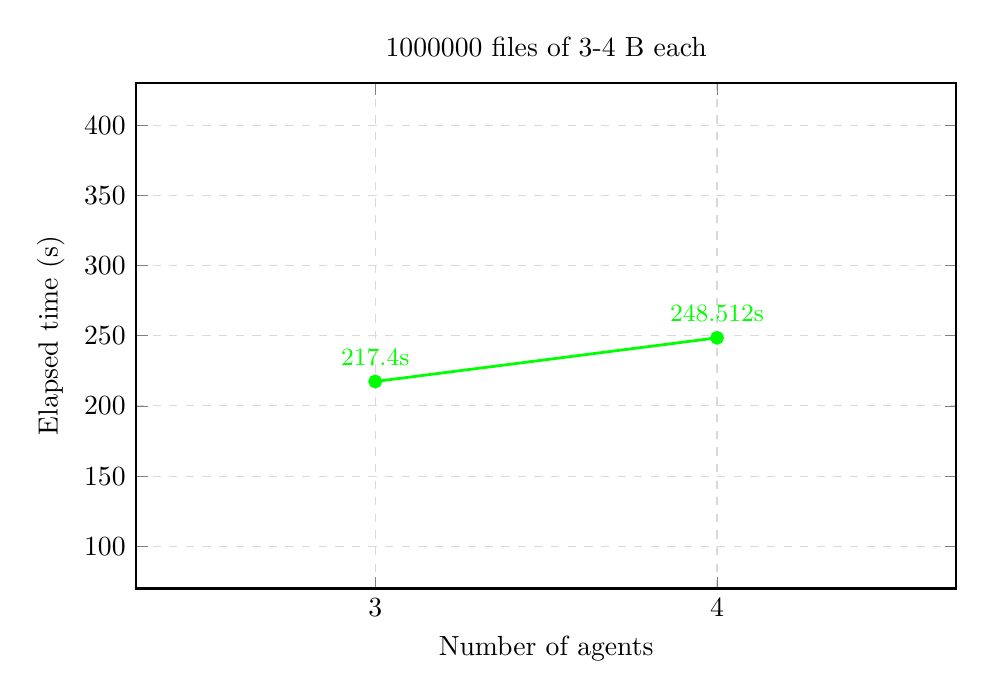
\begin{tikzpicture}
\begin{axis}[
    width=12cm, height=8cm,
    xlabel={Number of agents},
    ylabel={Elapsed time (s)},
    xmin=2.5, xmax=4.5,
    ymin=100, ymax=400,
    xtick={3,4},
    ytick={100,150,200,250,300,350,400},
    grid=major,
    grid style={dashed,gray!30},
    thick,
    title={1000000 files of 3-4 B each},
    enlargelimits=0.1,
    clip=false,
    nodes near coords,
    every node near coord/.append style={font=\small, anchor=south, yshift=2pt},
    point meta=explicit symbolic
]

\addplot[color=green, mark=*, line width=1pt] coordinates {
    (3,217.4) [217.4s]
    (4,248.512) [248.512s]
};
\end{axis}
\end{tikzpicture}
\caption{Elapsed time for very large datasets.}
\label{fig:test-4}
\end{figure}
